\chapter{Gruppierung von Nutzern anhand der verwendeten Wörter }
\label{chap:cluster_hashtags}
Es scheint offensichtlich, das wenn wir über ein bestimmtes Thema diskutieren auch bestimmt Wörter benutzten, um uns überhaupt mit dem Thema auseinander setzen zu können. Eine Diskussion über den Klimawandel scheint schwer praktikabel, ohne auch nur einmal das Wort "{}Klimawandel"{} zu benutzten. Diese, schon fast als Axiom betrachtbare Tatsache soll nun als Fundament für folgende These gelten: Bei Menschen, welche über ein bestimmtes Themen sprechen, deckt sich die Auswahl der verwendeten Wörter eher als bei Menschen, welche präferiert über andere Themen diskutieren. Diese Hypothese legt also nahe, dass Texte, welcher sich mit dem Klimawandel auseinandersetzt sich untereinander in der Wortwahl weniger unterscheiden als wenn man sie mit einem Text über den Nahostkonflikt vergleicht.

\section{Berechnung der Ähnlichkeit von Texten}
\label{chap:berechnung_texteahnlichkeit}
Um die Ähnlichkeit der Worte nun vergleichen zu können, muss zunächst ein Kriterium oder eine Maßzahl gefunden und anschließend berechnet werden, anhand der die Texte verglichen werden können. Distanzfunktionen kennt man vor allem aus der Geometrie. Hier ist ein häufiger Vertreter die Euklidische Distanz. \\ \newline
Eine hierfür geeignete Methodik hierzu ist die Berechnung der Kosinus-Distanz \footfullcite[2]{Godfrey.21.08.2014}. Sind die Merkmale zweier zu vergleichenden Merkmalsträger als n-dimensionaler Vektor vorhanden, so bestimmt die Kosinus-Distanz den Winkel zwischen diesen beiden Vektoren. Die Euklidische-Distanz jedoch  bestimmt die Abstand zwischen den beiden Enden der Vektoren. Außerdem ist die Kosinus-Distanz schneller zu berechnen und berechnet die Abstände zwischen zwei Texten unabhängig von deren Länge, im Gegensatz zur Euklidischen-Distanz.
\begin{equation}
	\begin{aligned} 
		\text{Berechnung der Kosinus-Distanz}&& 
		\cos(\alpha)&=\frac{x\cdot y}{\left|x\right|\cdot \left|y\right|} \\
		\text{Berechnung der Euklidischen Distanz}&& 
		{d}_{xy}&=\sqrt{\sum _{i=0}^{n}{\left|{x}_{i}-{y}_{i}\right|}^{2}} \\  
	\end{aligned} 
	\label{eq:distance}
\end{equation}

Die Formeln \eqref{eq:distance} zeigen die Berechnung der Kosinus-Distanz und der Euklidischen-Distanz zweier Vektoren im n-dimensionalen Raum. Um nun die Texte miteinander vergleichen zu können müssen für diese zunächst in Merkmalsvektoren überführt werden. \\ \newline
Da die Merkmale in diesem Kontext die verwendeten Wörter sind, braucht es einen Vektor, welcher beschreibt, ob ein bestimmtes Wort in einem Text enthalten ist oder nicht. Dazu müssen zuerst alle Wörter bestimmt werden, welche in der Summe $W_{acc}$ aller verwendeten Texte verwendet werden. Diese bilden die Summe aller möglichen Merkmale. Anschließend wird überprüft, welcher der Worte, welche über alle Texte hinweg existieren in den einzelnen Texten wieder gefunden werden. Dies soll nun anhand des Satzes $A$ "`Marc isst gerne Bananen"' und des Satzes $B$ "`Bananen kauft Lea gerne"' dargestellt werden. Die Menge $W_{x}$ stellt die Menge der im Satz enthaltenen Wörter dar. 
\begin{equation}
	\begin{aligned} 
		\text{Satz A}&& W_{A}&=\{\text{Marc},\text{isst},\text{gerne},\text{Bananen}\}  \\
		\text{Satz B}&& W_{B}&=\{\text{Bananen},\text{kauft},\text{Lea},\text{gerne}\}  \\
		\text{Vereinigung}&& W_{acc} &= W_{A}\cup W_{B} = \{\text{Marc},\text{isst},\text{gerne},\text{Bananen},\text{kauft},\text{Lea}\}  \\
	\end{aligned} 
	\label{eq:satz}
\end{equation}
Aus der Formel \eqref{eq:satz} ergeben sich die Wortmengen der einzelnen Sätze sowie die Vereinigung aller Wortmengen. Um diese Wortmengen zu überprüfen wird nun für jedes Wort $w$ in $W_{acc}$ geprüft, ob $w$ in der Wortmenge des Satzes $W_{x}$ enthalten ist. 


\begin{center}
	\begin{table}
	\begin{tabular}{c | c | c | c | c | c | c}
		
		$w$ aus $W_{acc}$ & Marc 	& isst 		& gerne 	& Bananen 	& kauft 	& Lea		\\
		\hline
		\hline
		$w\in {W}_{A}$ 	  & ja (1)	& ja (1)	& ja (1)	& ja (1)	& nein (0)	& nein (0)	\\
		\hline
		$w\in {W}_{B}$ 	  & nein (0)& nein (0)	& ja (1)	& ja (1)	& ja (1)	& ja (1)

	\end{tabular}
		\caption{Überführung von Wortmengen zu Vektoren für einzelne Nutzer}
	\end{table}
\end{center}

Somit ergibt sich aus den Zeilen der Tabelle für die Beiden Sätze A und B folgende Merkmalsvektoren

\begin{equation}
	\begin{aligned} 
		\text{Merkmalsvektor A}&& V_{A}&=\{1,1,1,1,0,0\}  \\
		\text{Merkmalsvektor B}&& V_{B}&=\{0,0,1,1,1,1\}
	\end{aligned} 
\label{eq:merkmalsvektoren}
\end{equation}
Auf diese Lassen sich nun die Distanzfunktionen anwenden. So würde die Kosinusdistanz 

\section{Verifikation der Ähnlichkeitsanalyse}
Die am Anfang des Kapitels getroffene Überlegungen legen nahe, dass Texte, welche sich mit dem gleichen Thema beschäftigen, eine ähnliche Auswahl von Wörtern verwenden. Genau dieses Phänomen soll hier in einer Stichprobe von vier Texten untersucht werden. Bei diesen handelt es sich um Artikel der Tagesschau, drei zum Thema Klimawandel und einer zum Thema Nahostkonflikt. Konkret sind es die Artikel unter den Titeln "`Deutschland soll "`klimafest"' werden"' \footfullcite[]{tag_klima_klimafest}, "`Klimawandel bleibt größte Gefahr"' \footfullcite[]{tag_klima_gefahr} und "`Wo der Klimawandel längst Realität ist"' \footfullcite[]{tag_klima_realiteat} zum Thema Klimawandel und der Artikel "Die Gewalt nimmt nicht ab"' \footfullcite[]{tag_nahost}, welcher sich mit dem Nahostkonflikt beschäftigt. \\ \newline
Mithilfe der im \autoref{chap:berechnung_texteahnlichkeit} mathematischen Grundlage soll nun unter Verwendung der Kosinus-Distanz die Ähnlichkeit der Texte zueinander in einer Matrix dargestellt werden. Um diese These zu beweisen, muss nun eine Methode entwickelt werden, um die Ähnlichkeit der Texte darzustellen. Dabei müssen sich die drei ersteren Texte, welche alle das Thema Klimawandel behandeln, untereinander Ähnlich sein. Zudem müssen sie zum vierten Text mit dem Thema Nahostkonflikt unterscheiden. \\ \newline
Im nachfolgenden soll nun der Prozess dargestellt werden, mit welchem diese Unterscheidung realisiert wurde.
\section{Aufbereitung von Texten zur Ähnlichkeitsanalyse}
Ein großes Problem bei der semantischen Analyse von Texten ist der gering Informationsgehalt pro Wort. Die meisten Worte innerhalb eines Satzes dienen dem Menschen zwar zum besseren Verständnis und Einordnung des Textes, dienen aber nicht wirklich dem Inhalt des Textes. So sind zur Einordnung des Themas des Satzes "`Nun hat die Bundesregierung einen Aktionsplan vorgelegt"' nur die Wörter "`Bundesregierung"' und "`Aktionsplan"' von entschiedener Bedeutung. \\ \newline
Um das Rauchen in einem Satz nun zu verringern, muss man zunächst alle Wörter herausfiltern, welche nicht maßgeblich zur Semantik des Satzes beitragen. Diese Art der Wörter, unter welchen vor allem Personal- und Possessivpronomen fallen, werden allgemein Stoppwörter genannt. Im Kontext dieser Arbeit wurde eine sehr erweiterte Liste an Stoppwörtern verwendet, welche sich unter folgenden Link finden lässt: \url{https://github.com/solariz/german_stopwords/}. \\ \newline
Zudem sind durch die Regeln der Grammatik eigentlich gleiche Wörter innerhalb unterschiedlich Sätze in unterschiedlichen Kasus wiederzufinden. Auch unterschiedliche Tempora führen zu einer Abänderung der Wortstämme. So sollten die Wörter "`demonstrieren"' und "`demonstrierte"' zusammengeführt werden. \\ \newline
Um in einen Text also weiter das Rauchen zu verringern, müssen die einzelnen Wörter auf ihren Wortstamm zurückgeführt werden. Dieser Prozess heißt Lemmatisierung. Für Deutsche Texte gibt es hierfür unterschiedliche Bibliotheken für Python, welche im Nachfolgenden verglichen werden sollen: \\ \newline

%TODO vergleiche Tagger

Aus dem Vergleich ergibt sich, dass der HanoverTagger am besten für die Aufgabe verwendbar ist. \\ \newline

Die Tabellen in Abbildung \ref{fig:textvergleich} stellen das Ergebnis der nun besprochenen Methodik dar. Jede Zelle der Tabelle stellt dar, wie Ähnlich sich Text A, welcher aus der Spalte entnommen werden kann und Text B, welcher durch die Zeile angegeben ist, sind. Mit jeder Tabelle ein Prozessschritt eingeführt. So werden in Tabelle (b) die Stoppwörter herausgefiltert, in Tabelle (c) wird zudem noch die Wortstandrückführung durchgeführt. Zur besseren Visualisierung wurden die Zellen abhängig vom Ähnlichkeitswert eingefärbt: Der höchste Wert wird grün gefärbt, werden der niedrigste Wert rot markiert wird. Die Farbwerte der restlichen Zellen werden über eine lineare Interpolation und additive Farbmischung bestimmt.\\ \newline
Die vier Tabellen zeigen die Sinnhaftigkeit jedes Schrittes eindeutig auf: Während in der Tabelle ganz oben das Ergebnis noch alles andere als das gewünschte ist, werden die Texte in Tabelle (d) eindeutig nach Thema unterscheidbar. So sieht man, dass  in Tabelle (a)  der Text "`Wo der Klimawandel längst Realität ist"' dem Text "`Nahostkonflikt: Die Gewalt nimmt nicht ab"' mit einem Wert von 0.023 ähnlicher ist als dem Text "`Klimawandel bleibt größte Gefahr"' mit dem Wert 0.219. In Tabelle (d) werden die beiden Texte zum Thema Klimawandel deutlich von dem dritten Text unterschieden. 
\begin{figure}
	\centering
	\subfloat[Ohne Datenaufbereitung]{%
		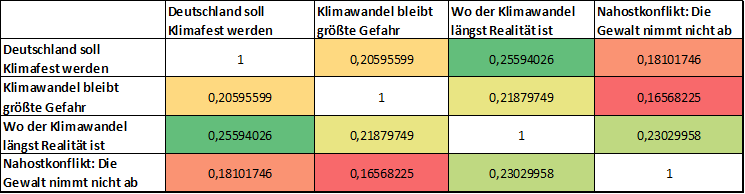
\includegraphics[clip,width=\linewidth]{images/tabelle_abstand_artikel_1.png}%
	}

	\subfloat[Mit Herausfiltern der Stoppwörter]{%
		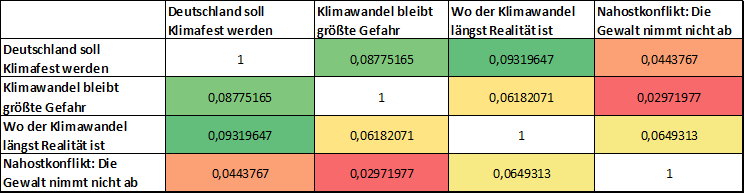
\includegraphics[clip,width=\linewidth]{images/tabelle_abstand_artikel_2.png}%
	}

	\subfloat[Mit Herausfiltern der Stoppwörter und Wortstammrückführung]{%
		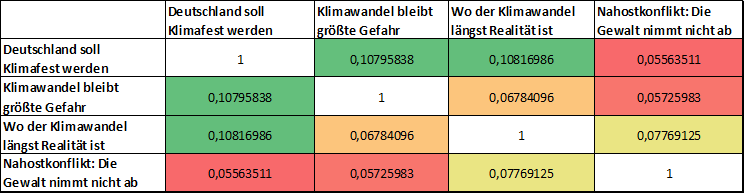
\includegraphics[clip,width=\linewidth]{images/tabelle_abstand_artikel_3.png}%
	}

	\subfloat[Mit Herausfiltern der Stoppwörter, Wortstammrückführung und Minimalanzahl für Wort]{%
		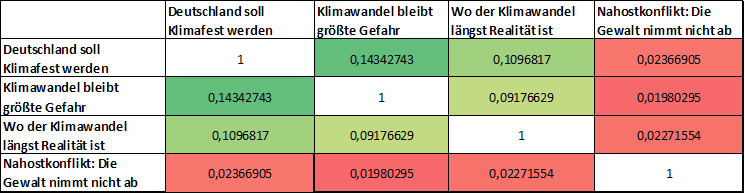
\includegraphics[clip,width=\linewidth]{images/tabelle_abstand_artikel_4.png}%
	}
	\caption{Ähnlichkeitsmaße der einzelnen Artikel unter Verwendung der Kosinus-Distanz}
	\label{fig:textvergleich}
\end{figure}

\section{Berechnung der Merkmalsvektoren der Nutzer}
Nun muss der Prozess, der bei Tagesschauartikeln funktioniert auf die einzelnen Nutzer angewendet werden. Ziel ist die Erstellung eines Merkmalsvektoren analog zu dem aus Formel \ref{eq:merkmalsvektoren}. 


\section{Aufteilen der Nutzer in Cluster}
In den vorausgehenden Kapiteln wurde dargestellt, wie aus den 


 
